\documentclass[12pt]{article}
\usepackage[margin=2.5cm]{geometry}
\usepackage{enumerate}
\usepackage{amsfonts}
\usepackage{amsmath}
\usepackage{fancyhdr}
\usepackage{amsmath}
\usepackage{amssymb}
\usepackage{amsthm}
\usepackage{mdframed}
\usepackage{graphicx}
\usepackage{subcaption}
\usepackage{adjustbox}
\usepackage{listings}
\usepackage{xcolor}
\usepackage{booktabs}
\usepackage[utf]{kotex}
\usepackage{hyperref}
\usepackage{accents}

\definecolor{codegreen}{rgb}{0,0.6,0}
\definecolor{codegray}{rgb}{0.5,0.5,0.5}
\definecolor{codepurple}{rgb}{0.58,0,0.82}
\definecolor{backcolour}{rgb}{0.95,0.95,0.92}

\lstdefinestyle{mystyle}{
    backgroundcolor=\color{backcolour},
    commentstyle=\color{codegreen},
    keywordstyle=\color{magenta},
    numberstyle=\tiny\color{codegray},
    stringstyle=\color{codepurple},
    basicstyle=\ttfamily\footnotesize,
    breakatwhitespace=false,
    breaklines=true,
    captionpos=b,
    keepspaces=true,
    numbers=left,
    numbersep=5pt,
    showspaces=false,
    showstringspaces=false,
    showtabs=false,
    tabsize=1
}

\lstset{style=mystyle}

\pagestyle{fancy}
\renewcommand{\headrulewidth}{0.4pt}
\lhead{CSC 343}
\rhead{Worksheet 11 Solution}

\begin{document}
\title{CSC343 Worksheet 11 Solution}
\maketitle

\begin{enumerate}[1.]
    \item

    \begin{enumerate}[a)]
        \item

    \begin{lstlisting}[language=XML]
    <? xml version = "1.0" encoding = "utf-8"?>
    <xsl:stylesheet xmlns:xsl = "http://www.w3.org/1999/ISL/Transform">
        <xsl:template match = "/">
            <html>
                <BODY>
                    <H1>Manufacturerers</h1>
                    <OL>
                        <xsl:for-each select="Products/Maker">
                            <Li><xsl:value-of select="@name"/></li>
                        </xsl:for-each>
                    </ol>
                </body>
            </html>
        </xsl:template>
    </xsl:stylesheet>
    \end{lstlisting}


        \bigskip

        \underline{\textbf{Notes:}}

        \bigskip

        \begin{itemize}
            \item XLST
            \begin{itemize}
                \item Also means \textbf{Extensible Stylesheet Language for Transformation}
                \item Allows to transform XML documentes into HTML
                \item Is another language
            \end{itemize}
            \item XLST Basics

            \bigskip

            \textbf{Syntax:}

            \bigskip

            $<$? xml version = "1.0" encoding = "utf-8"?$>$

            $<$xsl:stylesheet xmlns:xsl = "http://www.w3.org/1999/ISL/Transform"$>$

            \quad...

            $<$/xsl:stylesheet$>$


            \item Templates

            \bigskip

            \underline{\textbf{Example:}}

    \begin{lstlisting}[language=XML]
    <? xml version = "1.0" encoding = "utf-8"?>
    <xsl:stylesheet xmlns:xsl = "http://www.w3.org/1999/ISL/Transform">
        <xsl:template match = "/">
            <HTML>
                <BODY>
                    <B>This is text</b>
                </body>
            </html>
        </xsl:template>
    </xsl:stylesheet>
    \end{lstlisting}

            \item Obtaining values from XML Data
            \begin{itemize}
                \item value-of
                \begin{itemize}
                    \item Is used to extract the value of a selected node.
                    \item \textbf{Syntax:} $<$xsl value-of select = "\textit{expression}" /$>$


                    \bigskip

                    \underline{\textbf{Example:}}

    \begin{lstlisting}[language=XML]
    <? xml version = "1.0" encoding = "utf-8"?>
    <xsl:stylesheet xmlns:xsl = "http://www.w3.org/1999/ISL/Transform">
        <xsl:template match="/Movies/Movie">
            <xsl:value-of select = "@title"/>
        </xsl:template>
    </xsl:stylesheet>
    \end{lstlisting}
                \end{itemize}

                \item Apply-templates
                \begin{itemize}
                    \item applies a $<$xls:template$>$ to the current element or
                    to the current element's child nodes.
                    \begin{itemize}
                        \item select='.' means choose the current value
                    \end{itemize}
                \end{itemize}

                \begin{center}
                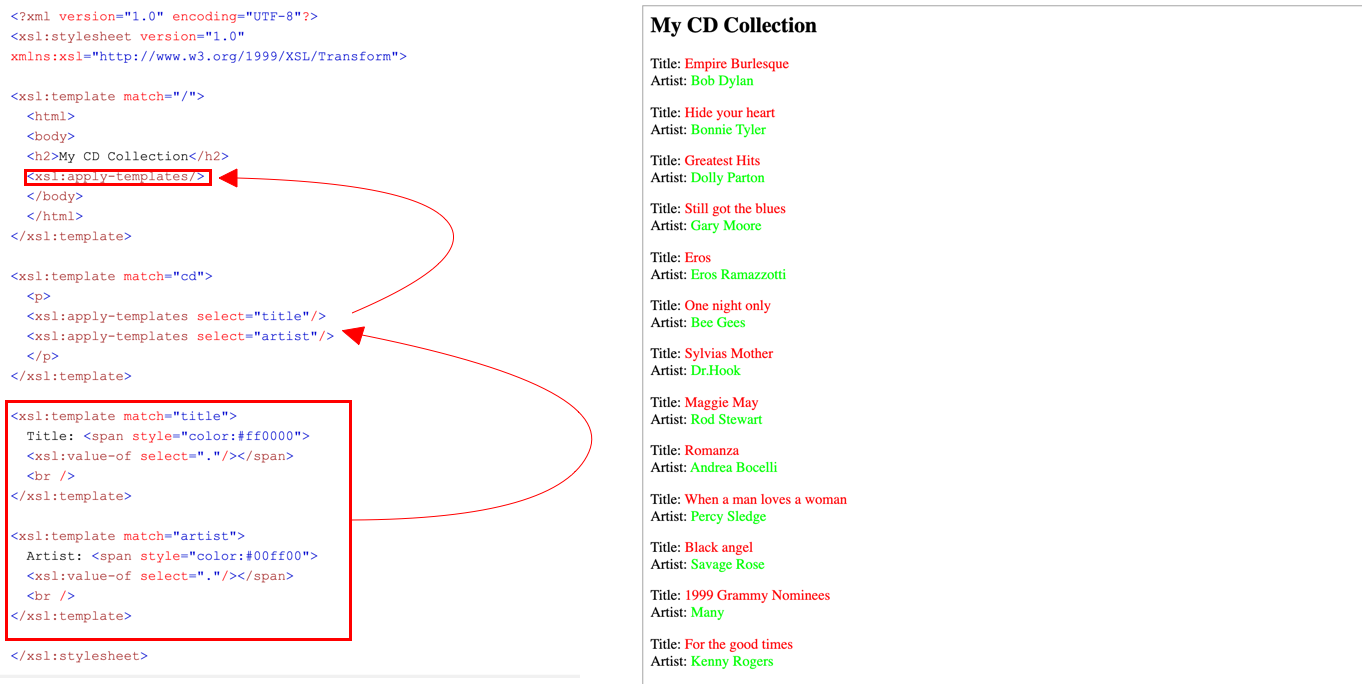
\includegraphics[width=\linewidth]{images/worksheet_11_solution_1.png}
                \end{center}

                \item For-loop in XSLT
                \begin{itemize}
                    \item \textbf{Syntax:} $<$xsl:for-each select = "\textit{expression}" $>$ ... $<$/xsl:for-each$>$
                    \item Is easier to maintain and read than apply templates $^{[1]}$
                \end{itemize}

                \begin{center}
                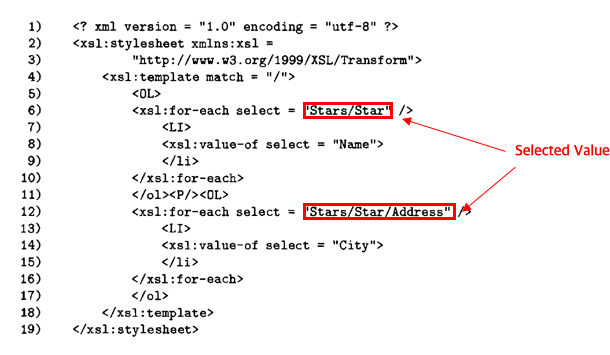
\includegraphics[width=0.7\linewidth]{images/worksheet_11_solution_2.png}
                \end{center}

                \bigskip

                \underline{\textbf{References:}}

                \bigskip

                \begin{enumerate}[1)]
                    \item StackOverflow, differences between for-each and templates in xsl?, \href{https://stackoverflow.com/questions/4460232/differences-between-for-each-and-templates-in-xsl}{link}
                \end{enumerate}
            \end{itemize}

            \item If condition in XSLT
            \begin{itemize}
                \item \textbf{Syntax:} $<$xsl:if test = "\textit{boolean expression}"$>$
            \end{itemize}

            \begin{center}
            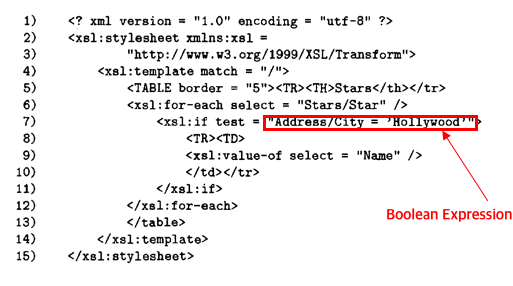
\includegraphics[width=0.7\linewidth]{images/worksheet_11_solution_3.png}
            \end{center}
        \end{itemize}

        \item

    \begin{lstlisting}[language=XML]
    <? xml version = "1.0" encoding = "utf-8"?>
    <xsl:stylesheet xmlns:xsl = "http://www.w3.org/1999/ISL/Transform">
        <xsl:template match = "/">
            <html>
                <BODY>
                    <TABLE>
                        <TH>
                            <TD>Model</td>
                            <TD>Price</td>
                        </th>
                        <xsl:for-each select="Products/Maker">
                            <TR>
                                <TD>
                                    <xsl:value-of select="@model"/>
                                </td>
                                <TD>
                                    <xsl:value-of select="@price"/>
                                </td>
                            </tr>
                        </xsl:for-each>
                    </table>
                </body>
            </html>
        </xsl:template>
    </xsl:stylesheet>
    \end{lstlisting}


    \end{enumerate}
\end{enumerate}

\end{document}